\documentclass[12pt]{article} 
\usepackage[utf8]{inputenc}
\usepackage{amssymb, amsmath, amsthm, amsfonts}
\usepackage{euscript}
\usepackage{graphicx}
\usepackage[dvipsnames]{xcolor}
\usepackage{titlesec}
\newcommand{\sectionbreak}{\clearpage}
\usepackage{url}
\usepackage{hyperref}
\hypersetup{colorlinks=true, urlcolor=RoyalBlue, citecolor=RedViolet, linkcolor=black}
\usepackage{pdfpages}
\usepackage{array}
\usepackage[margin=1in]{geometry}
\usepackage{enumitem}
\usepackage{setspace} 
%\setlength\parindent{0pt}
\linespread{1.2}
\newtheorem*{theorem}{Theorem}
\newtheorem*{prop}{Proposition}
\theoremstyle{definition} 
\newtheorem*{definition}{Definition}
%\renewcommand{\familydefault}{\sfdefault}
\newcommand{\R}{\mathbb{R}} %the reals
\newcommand{\Q}{\mathbb{Q}} %the rationals
\newcommand{\N}{\mathbb{N}} %the natural numbers
\newcommand{\Z}{\mathbb{Z}} %the integers
\newcommand{\eps}{\varepsilon} %a cooler epsilon
\renewcommand{\emptyset}{\varnothing}
\newcommand{\solution}{\textcolor{PineGreen}{Solution:\newline}}
%%%%% End of preamble %%%%%

\begin{document}

\begin{titlepage}
\begin{center}
    \LARGE{Math 3100 Final Portfolio}
    
    \bigskip
    
    \Large{Zachary A. Hampton}
    
    \medskip
    
    \Large{Fall 2024}
\end{center}

 \vfill
    
    \begin{figure}[h]
        \centering
        
\includegraphics[width=.8\textwidth]{fractology_11_ZAHAMPTON.jpg}
        \caption{Fractology 11 by Zachary A. Hampton (2015) \cite{Flower08}}
        \label{fig:my_label}
    \end{figure}
    
    \vfill
\end{titlepage}

\tableofcontents

%------------Project Reflection -------------

\section{Project Reflection}

As a computer science major with a strong interest in mathematics, this proof-writing course provided an opportunity to sharpen my understanding of logical reasoning and systematic thinking—skills. While my recent class in discrete mathematics introduced me to concepts like logical operators, set theory, and some basic proofs, this course demanded a new whole new level of understanding from me. Instead of just identifying and solving mathematical structures, I had to construct and communicate them clearly and precisely from first basic principles.

The portfolio project was particularly transformative in this regard. Problem 1, which involved proving the biconditional relationship between even integers and divisibility by 4, challenged me to approach mathematical reasoning differently. Initially, the problem seemed straightforward, but constructing a proof revealed its complexities. Breaking down the problem, defining terms like "even" and "divisible," and carefully justifying every step were essential. This experience reminded me of debugging and refining code in programming—ensuring every assumption and step aligns to create a complete solution.

Through this process, I realized the importance of clarity and precision in mathematical writing. Early drafts of my proofs often omitted key justifications or used vague language, making the arguments less convincing. Revising these drafts taught me to be explicit about assumptions and intentional in structuring arguments. This mirrors my experience in programming, where clean, well-documented code is just as important as functional correctness. I feel like the process of revising proofs improved my ability to communicate ideas effectively.

Another valuable insight from the course was the shift in how I view mathematics. Previously, I thought of “doing math” as solving problems using formulas and plugging in numbers. This course re-framed it as a process of exploration and justification, where the reasoning itself is as important as the result. For example, in Problem 2, which explored $a^2=b^3$ and divisibility, I learned that the journey of constructing a logical argument can reveal deeper patterns and relationships that go beyond the immediate problem.

This course also enhanced my problem-solving strategies. Tackling complex proofs required breaking problems into manageable components and connecting them together in a systematic way. This approach aligns with algorithm design in computer science, where problems are deconstructed into logical steps before being implemented. Also, the emphasis on reflecting and iterating on my work has reinforced the importance of learning from mistakes and improving over time.

One of the most rewarding aspects of this course has been seeing how mathematical reasoning connects to other areas of study. The ability to construct rigorous arguments is fundamental in data science, where proving the validity of a model or justifying an approach is critical. Similarly, the logical skills developed here will enhance my work in computer engineering, whether in designing algorithms or verifying system correctness.

Looking ahead, I see this course as a important experience that will continue to influence my future academic and professional pursuits. For new students to the course, my advice is to not be instantly scared and say you hate proofs; you need to embrace the process of learning this different type of writing. Don’t rush to the solution, instead focus on understanding the problem and constructing a clear, logical argument. While I decided to do the portfolio projects, collaboration and feedback can also be completely invaluable; discussing ideas with peers can often provide new insights and highlights areas where you can improve.

In summary, this proof-writing course has significantly deepened my understanding of mathematical reasoning and its applications. It has enhanced my ability to think critically, write clearly, and solve problems systematically, skills that are vital not only in mathematics but across all areas of disciplines. I personally would like to thank Dr. Johnson for making this my favorite class of the semester; I'm sad to say that it's my last official math class for the foreseeable future, but I'm grateful to have such good memories to part with.

\newpage

%------------Problem 1 -------------

\section{Portfolio Problem 1}

\subsection{Introductory Material and Definitions} 

To prove the statement, "For each integer \( n \), \( n \) is even if and only if 4 divides \( n^2 \)," we will use the following standard definitions:

\begin{itemize}
    \item \textbf{Even integer:} An integer \( n \) is even if there exists an integer \( k \) such that \( n = 2k \).
    \item \textbf{Odd integer:} An integer \( n \) is odd if there exists an integer \( k \) such that \( n = 2k + 1 \).
    \item \textbf{Divisibility:} For integers \( a \) and \( d \), we say \( d \) divides \( a \) (written \( d \mid a \)) if there exists an integer \( m \) such that \( a = dm \).
    \item We will also make use of basic modular arithmetic facts, such as if \( 4 \mid n^2 \), then \( n^2 \equiv 0 \pmod{4} \).
\end{itemize}

These definitions provide the framework for analyzing parity (evenness/oddness) and examining when a square is divisible by 4.

\subsection{Examples} 

Before constructing a proof of the biconditional statement, we first consider several concrete instances to gain intuition.

First, we check whether squaring an even integer always produces a number divisible by 4. For instance, if we take \(a = -2\), which is even, then \(a^2 = (-2)^2 = 4\). Since \(4 \mid 4\), this example supports the forward direction of our statement. Similarly, if we let \(a = 0\), then \(0^2 = 0\), and clearly \(4 \mid 0\). For \(a = 2\), we have \(2^2 = 4\), and again \(4 \mid 4\). Finally, if we choose \(a = 4\), then \(4^2 = 16\), and \(4 \mid 16\). These examples demonstrate that when we start with an even integer, its square is indeed divisible by 4.

Next, we examine squares that are known to be multiples of 4 and check if their square roots are even. Consider \(b = 0\). Since \(0 = 0^2\) and \(4 \mid 0\), we see that the integer whose square is 0 is \(0\), which is even. If \(b = 4\), then \(4 = 2^2\), and since \(4 \mid 4\), the corresponding integer \(2\) is even. If \(b = 16\), then \(16 = 4^2\), and \(4 \mid 16\) with the original integer \(4\) being even. Finally, let \(b = 144\). We have \(144 = 12^2\), and \(4 \mid 144\). The integer whose square is 144 is 12, which is even. These examples confirm that if a square is divisible by 4, the original number must be even.

Together, these examples align with the biconditional statement, providing confidence in its validity before proceeding to a formal proof.

\newpage

\subsection{Final Draft}

\begin{theorem}
    For each integer \( n \), \( n \) is even if and only if 4 divides \( n^2 \).
\end{theorem}

\begin{proof}
    Let \( n \) be an integer. To prove the biconditional statement, "\( n \) is even if and only if 4 divides \( n^2 \)", we must prove the if/then statement in both the forward and reverse directions.

    \vspace{1em}

    For the forward direction, we assume \( n \) is even, and we will prove that \( 4 \mid n^2 \). By the definition of even, there exists an integer \( k \) such that \( n = 2k \). Substituting for \( n \) into \( n^2 \), we get:
    \begin{align*}
        n^2 &= (2k)^2 \\
             &= 4k^2 \\
             &= 2(2k^2).
    \end{align*}

    We find that \( 2k^2 \) is an integer due to closure under multiplication. Thus, \( n^2 = 4k^2 \), which shows that \( n^2 \) is divisible by 4, since 4 divides \( 4k^2 \) by the definition of divisibility. Therefore, we have proven that if \( n \) is even, then \( 4 \mid n^2 \).

    \vspace{1em}
    For the reverse direction, we assume \( 4 \mid n^2 \) and proceed by contradiction. By the definition of congruence mod \( n \), we can write \( 4 \mid n^2 \) as:
    \[
    n^2 \equiv 0 \pmod{4}.
    \]
    Now, suppose \( n \) is odd. By the definition of odd, \( n = 2k + 1 \) for some \( k \in \mathbb{Z} \). Substituting for \( n \) into \( n^2 \), we get:
    \begin{align*}
        n^2 &= (2k + 1)^2 \\
             &= 4k^2 + 4k + 1 \\
             &= 4(k^2 + k) + 1.
    \end{align*}
    So, \( n^2 = 4(k^2 + k) + 1 \), which implies that \( n^2 \equiv 1 \pmod{4} \). However, we assumed that \( n^2 \equiv 0 \pmod{4} \). Thus, our assumption that \( n \) is odd must be false, and it follows that \( n \) is even.

    \vspace{1em}
    
    Therefore, we have proven that \( n \) is even if and only if \( 4 \mid n^2 \).
\end{proof}

\noindent Include additional proposition and proof environments as needed.

\noindent Reminder: Include citations for any material from any source including collaborations \cite{Collab1}, the textbook \cite{Sund21}, or other sources \cite{Whatever24}

%------------Problem 2 -------------

\section{Portfolio Problem 2}

\subsection{Introductory Material and Definitions}

For the proposition: "If \( a^2 = b^3 \) and \( a \) is even, then \( 4 \mid a \)," we will use:

\begin{itemize}
    \item The definition of even integers as above.
    \item The definition of divisibility as above.
    \item Basic properties of even and odd integers, such as: if \( n^2 \) is even, then \( n \) is even.
    \item The fact that if \( b^3 \) is divisible by 4, then \( b \) must be even (since an odd integer raised to any power remains odd).
\end{itemize}

These definitions and facts allow us to unravel the structure of \( a^2 = b^3 \) and deduce conditions on \( a \).

\subsection{Examples}

For the second proposition, we seek to understand the relationship between \(a^2 = b^3\) and the evenness of \(a\). Specifically, we want to show that if \(a^2 = b^3\) and \(a\) is even, then \(4 \mid a\).

To explore this, we consider explicit pairs \((a, b)\) that satisfy \(a^2 = b^3\) and for which \(a\) is even. One such pair is \(a = 8\) and \(b = 4\), since \(8^2 = 64\) and \(4^3 = 64\). Here, \(a = 8\) is even, and indeed \(4 \mid 8\). Another example is \(a = 64\) and \(b = 16\), because \(64^2 = 4096\) and \(16^3 = 4096\). In this case, \(a = 64\) is even, and \(4 \mid 64\).

A third example is \(a = 216\) and \(b = 36\) where \(216^2 = 46656\) and \(36^3 = 46656\). The integer \(216\) is even, and it is divisible by 4. Finally, consider \(a = 512\) and \(b = 64\). Since \(512^2 = 262144\) and \(64^3 = 262144\), the condition \(a^2 = b^3\) holds. The integer \(512\) is even, and \(4 \mid 512\).

In each of these cases, whenever \(a^2 = b^3\) holds and \(a\) is even, it turns out that \(a\) is not just even but divisible by 4. These examples suggest the deeper property we aim to prove, reinforcing the idea that the condition \(a^2 = b^3\) imposes a certain structural factorization on \(a\) that ensures divisibility by 4.

\newpage

\subsection{Final Draft of Proof}

\textbf{Proposition:} Let \( a, b \in \mathbb{N} \). If \( a^2 = b^3 \) and \( a \) is even, then \( 4 \mid a \).

\begin{proof}
    Assume \( a \) and \( b \) are natural numbers. We will prove that if \( a^2 = b^3 \) and \( a \) is even, then \( 4 \) divides \( a \). Since \( a \) is even, there exists an integer \( k \) such that \( a = 2k \). Substituting \( a = 2k \) into \( a^2 \), we get:
    \[
    a^2 = (2k)^2 = 4k^2.
    \]

    By the hypothesis \( a^2 = b^3 \), it follows that:
    \[
    b^3 = 4k^2.
    \]

    Since \( b^3 \) is divisible by \( 4 \), it follows that \( b^3 \) is even. By previous results, \( n^3 \) is even if and only if \( n \) is even, so \( b \) must also be even. Thus, there exists an integer \( m \) such that \( b = 2m \). Substituting \( b = 2m \) into \( b^3 \), we have:

    \[
    b^3 = (2m)^3 = 8m^3.
    \]

    Thus, the equation becomes:
    \begin{align*}
        4k^2 & = 8m^3, \\
        k^2 & = 2m^3.
    \end{align*}

    By previous results, since \( k^2 \) is even, \( k \) must also be even. Let \( k = 2n \) for some integer \( n \). Recalling that \( a = 2k \), we substitute \( k = 2n \) into the expression for \( a \), and we have:  
    \[
    a = 2(2n) = 4n.
    \]

    Therefore, \( a \) is divisible by \( 4 \), which proves the proposition that if \( a^2 = b^3 \) and \( a \) is even, then \( a \) must be divisible by \( 4 \).
\end{proof}

%------------Appendices -------------

\appendix

%------------ Problem 1 Rough Drafts -------------

\section{Appendix: Problem 1 Rough Drafts}

\subsection{Examples and Definitions}

\textbf{Problem to prove:} Construct both a know-show table and a first attempt at a formal proof of the following biconditional statement.

\begin{prop}
    For each integer \( n \), \( n \) is even if and only if 4 divides \( n^2 \).
\end{prop}

% Exploratory work

\textbf{Exploratory work/Examples:}
\begin{itemize}
    \item Find four even integers \( a \). At least one integer must be negative. Square each integer \( a \) and determine if 4 divides \( a^2 \).
    \begin{itemize}
        \item If we set \( a = -2 \), then \( (-2)^2 = 4 \), and \( 4 \mid 4 \).
        \item If we set \( a = 0 \), then \( 0^2 = 0 \), and \( 4 \mid 0 \).
        \item If we set \( a = 2 \), then \( 2^2 = 4 \), and \( 4 \mid 4 \).
        \item If we set \( a = 4 \), then \( 4^2 = 16 \), and \( 4 \mid 16 \).
    \end{itemize}
    
    \item Find four perfect squares, \( b \), such that \( 4 \mid b \). Then find the integer \( c \) such that \( b = c^2 \). Determine if \( c \) is even or odd.
    \begin{itemize}
        \item If we set \( b = 0 \), then \( 4 \mid 0 \). Using \( b = c^2 \), we get \( 0 = 0^2 \), so \( c = 0 \), which is even.
        \item If we set \( b = 4 \), then \( 4 \mid 4 \). Using \( b = c^2 \), we get \( 4 = 2^2 \), so \( c = 2 \), which is even.
        \item If we set \( b = 16 \), then \( 4 \mid 16 \). Using \( b = c^2 \), we get \( 16 = 4^2 \), so \( c = 4 \), which is even.
        \item If we set \( b = 144 \), then \( 4 \mid 144 \). Using \( b = c^2 \), we get \( 144 = 12^2 \), so \( c = 12 \), which is even.
    \end{itemize}
\end{itemize}

% Know-SHow table for Forward Direction

\newpage

\subsection{Know-Show Table: (Forward)}

If \( n \) is even, then \( 4 \mid n^2 \)

\begin{center}
    \begin{tabular}{|p{.1\textwidth}|p{.5\textwidth}|p{.3\textwidth}|}
    \hline
    \textbf{Step} & \textbf{Know} & \textbf{Reason} \\
    \hline
        P1 & \( n \) is even & Hypothesis \\
    \hline
        P2 & \( \exists k \in \mathbb{Z} \text{ s.t. } n = 2k \) & Definition of even \\
    \hline
        P3 & \( n^2 = (2k)^2 = 4k^2 \) & Substitution \\
    \hline
        P4 & \( 4k^2 = 2(2k^2) \) & Factoring out \( 2 \) \\
    \hline
        P5 & \( 2k^2 \in \mathbb{Z} \) & \( \mathbb{Z}\) closed under multiplication \\
    \hline
        P6 & \( n^2 = 2q \) where \( q \in \mathbb{Z} \) & Set \( q = k^2 \) \\
    \hline
        Q1 & 4 divides \( n^2 \) & Defn divides \\
    \hline
    \textbf{Step} & \textbf{Show} & \textbf{Reason} \\
    \hline
    \end{tabular}
\end{center}

% Know-Show table for Reverse Direction

\subsection{Know-Show Table: If \( 4 \mid n^2 \), then \( n \) is even (Reverse)}

\begin{center}
    \begin{tabular}{|p{.1\textwidth}|p{.55\textwidth}|p{.25\textwidth}|}
    \hline
    \textbf{Step} & \textbf{Know} & \textbf{Reason} \\
    \hline
        P1 & \( 4 \mid n^2 \) & Hypothesis \\
    \hline
        P2 & \( n^2 = 4m \) for some \( m \in \mathbb{Z} \) & Definition of divisibility \\
    \hline
        P3 & \( n^2 \equiv 0 \mod 4 \) & Definition of congruence \\
    \hline
        P4 & Assume \( n \) is odd & For contradiction \\
    \hline
        P5 & \( n = 2k + 1 \) for some \( k \in \mathbb{Z} \) & Definition of odd \\
    \hline
        P6 & \( n^2 = (2k + 1)^2 = 4k^2 + 4k + 1 \) & Expand and simplify \( n^2 \) \\
    \hline
        P7 & \( n^2 = 4(k^2 + k) + 1 \) & Factor out 4 \\
    \hline
        P8 & \( k^2 + k \in \mathbb{Z} \) & \( \mathbb{Z}\) closed under multiplication \\
    \hline
        P9 & \( n^2 \equiv 1 \mod 4 \) & \( 4(k^2 + k) \equiv 0 \mod 4 \) \\
    \hline
        P10 & Contradicts \( n^2 \equiv 0 \mod 4 \) & From P2, since \( n^2 = 4m \) \\
    \hline
        Q1 & \( n \) is even & Definition of even \\
    \hline
    \textbf{Step} & \textbf{Show} & \textbf{Reason} \\
    \hline
    \end{tabular}
\end{center}

\newpage

% First Draft

\subsection{First Draft}

%T Theorem

\begin{theorem}
    For each integer \( n \), \( n \) is even if and only if 4 divides \( n^2 \).
\end{theorem}

% Proof

\begin{proof}
    In order to prove this biconditional statement, we must prove the if/then statement in both the forward and reverse directions.

    \vspace{1em}

    For the forward direction, we assume \( n \) is even, and we will prove that \( 4 \mid n^2 \). By the definition of even, there exists an integer \( k \) such that \( n = 2k \). Substituting for \( n \) into \( n^2 \), we get:
    \[ n^2 = (2k)^2 = 4k^2 \]
    Then, we factor:
    \[ 4k^2 = 2(2k^2) \]
    We find that \( 2k^2 \) is an integer due to closure under multiplication. Now, we can write \( n^2 = 2q \), where \( q = 2k^2 \) is an integer, which shows that \( n^2 \) is divisible by 4. Therefore, we have proven that if \( n \) is even, then \( 4 \mid n^2 \).

    \vspace{1em}

    For the reverse direction, we assume \( 4 \mid n^2 \), and we will prove that \( n \) is even. By the definition of divides, there exists an integer \( m \) such that \( n^2 = 4m \). Because of the relationship with congruence, this can be restated as:
    \[ n^2 \equiv 0 \pmod{4} \]
    Due to integers not being closed under roots, we assume for contradiction that \( n \) is odd. By the definition of odd, \( n = 2k + 1 \) for some \( k \in \mathbb{Z} \). Substituting for \( n \) into \( n^2 \), we get:
    \[ n^2 = (2k + 1)^2 = 4k^2 + 4k + 1 \]
    Then, we factor:
    \[ 4k^2 + 4k + 1 = 4(k^2 + k) + 1 \]
    So, \( n^2 = 4(k^2 + k) + 1 \), which implies that, \( n^2 \equiv 1 \pmod{4} \). However, we assumed that \( 4 \mid n^2 \), which implies \( n^2 \equiv 0 \pmod{4} \). Therefore, our assumption that \( n \) is odd must be false, and it follows that \( n \) is even.
\end{proof}

\newpage

% Second Draft

\subsection{Second Draft}

\begin{theorem}
    For each integer \( n \), \( n \) is even if and only if 4 divides \( n^2 \).
\end{theorem}

\begin{proof}
    Let \( n \) be an integer. To prove the biconditional statement, "\( n \) is even if and only if 4 divides \( n^2 \)", we must prove the if/then statement in both the forward and reverse directions.

    \vspace{1em}

    For the forward direction, we assume \( n \) is even, and we will prove that \( 4 \mid n^2 \). By the definition of even, there exists an integer \( k \) such that \( n = 2k \). Substituting for \( n \) into \( n^2 \), we get:
    \begin{align*}
        n^2 &= (2k)^2 \\
             &= 4k^2 \\
             &= 2(2k^2)
    \end{align*}
    
    We find that \( 2k^2 \) is an integer due to closure under multiplication. Now, we can write \( n^2 = 2q \), where \( q = 2k^2 \) is an integer, which shows that \( n^2 \) is divisible by 4. Therefore, we have proven that if \( n \) is even, then \( 4 \mid n^2 \).

    \vspace{1em}

    For the reverse direction, we assume \( 4 \mid n^2 \), and we will prove that \( n \) is even. By the definition of divides, there exists an integer \( m \) such that \( n^2 = 4m \). Because of the relationship with congruence, this can be restated as:
    \[ n^2 \equiv 0 \pmod{4} \]
    Due to integers not being closed under roots, we assume for contradiction that \( n \) is odd. By the definition of odd, \( n = 2k + 1 \) for some \( k \in \mathbb{Z} \). Substituting for \( n \) into \( n^2 \), we get:
    \begin{align*}
        n^2 &= (2k + 1)^2 \\
             &= 4k^2 + 4k + 1 \\
             &= 4(k^2 + k) + 1
    \end{align*}
    So, \( n^2 = 4(k^2 + k) + 1 \), which implies that, \( n^2 \equiv 1 \pmod{4} \). However, we assumed that \( n^2 \equiv 0 \pmod{4} \). Thus, our assumption that \( n \) is odd must be false, and it follows that \( n \) is even.

    \vspace{1em}
    
    Therefore, we have proven that \( 4 \mid n^2 \) if and only if \( n \) is even.
\end{proof}
 
\newpage

\subsection{Reflection}

    \begin{itemize}
        \item My first draft doesn't declare n as an integer, so I added a sentence at the beginning of the first paragraph. 
        \item I decided to state what we're proving more clearly by referencing the theorem.
        \item Also, it was pointed out that I was restating something on lines 35 and 36, which I trimmed down.
        \item I stacked the math and aligned by the equation symbol. And I also restated the conclusion a little more clearly.\
        \item All-in-all, I think the proof is nearly dialed in, I'm excited for Dr. Johnson's critique.
    \end{itemize}


%------------ Problem 2 Rough Drafts -------------

\section{Appendix: Problem 2 Rough Drafts}

{Examples and Definitions}

\textbf{Problem to prove:} Construct both a know-show table and a first attempt at a formal proof of the following proposition.

\begin{prop}
    Let \( a, b \in \N \). If \( a^2 = b^3 \) and \( a \) is even, then \( 4 \mid a \).
\end{prop}

\subsection{Exploratory Work/Examples}

\textbf{Strategy:} 
To find four pairs of natural numbers \( (a, b) \) such that \( a^2 = b^3 \) and \( a \) is even, I modified my approach:
\begin{itemize}
    \item Filtered \( a \) to include only even numbers.
    \item Verified whether \( \sqrt[3]{a^2} \) is an integer and that \( b^3 = a^2 \).
    \item Added additional columns to check if \( a \) is even and ensure that both \( a \) and \( b \) satisfy the conditions for being natural numbers.
\end{itemize}

\textbf{Excel Formulas Used:}
\begin{itemize}
    \item Column A: Even natural numbers \( a \).
        \begin{itemize}
            \item Formula: \texttt{=even a value}
        \end{itemize}
    \item Column B: Squares of \( a \) (\( a^2 \)).
        \begin{itemize}
            \item Formula: \texttt{=POWER(A2, 2)}
        \end{itemize}
    \item Column C: Cube root of \( a^2 \) (\( \sqrt[3]{a^2} \)).
        \begin{itemize}
            \item Formula: \texttt{=POWER(B2, 1/3)}
        \end{itemize}
    \item Column D: Verification column for \( b^3 \) (\( b^3 \in \N \)).
        \begin{itemize}
            \item Formula: \texttt{=IF(AND(C2>0, C2=INT(C2)), C2*C2*C2 \& "$\in\mathbb{N}$", "b$\notin\mathbb{N}$")}
        \end{itemize}
    \item Column E: Even or Odd verification for \( a \).
        \begin{itemize}
            \item Formula: \texttt{=IF(A2=INT(A2), IF(MOD(A2,2)=0, "Even", "Odd"), "Not an Integer")}
        \end{itemize}
    \item Column F: Final check for Even and Natural.
        \begin{itemize}
            \item Formula: \texttt{=IF(AND(A2>0, A2=INT(A2), MOD(A2,2)=0, C2>0, C2=INT(C2)), "Natural and Even", "False")}
        \end{itemize}
\end{itemize}

\textbf{Results:} The four pairs satisfying \( a^2 = b^3 \), with \( a \) even, are:
\begin{center}
    \begin{tabular}{|c|c|c|c|}
    \hline
    \( a \) & \( a^2 \) & \( b \) & \( b^3 \) \\
    \hline
    8 & 64 & 4 & 64 \\
    64 & 4096 & 16 & 4096 \\
    216 & 46656 & 36 & 46656 \\
    512 & 262144 & 64 & 262144 \\
    \hline
    \end{tabular}
\end{center}

\textbf{Spreadsheet Screenshot:}
\begin{center}
    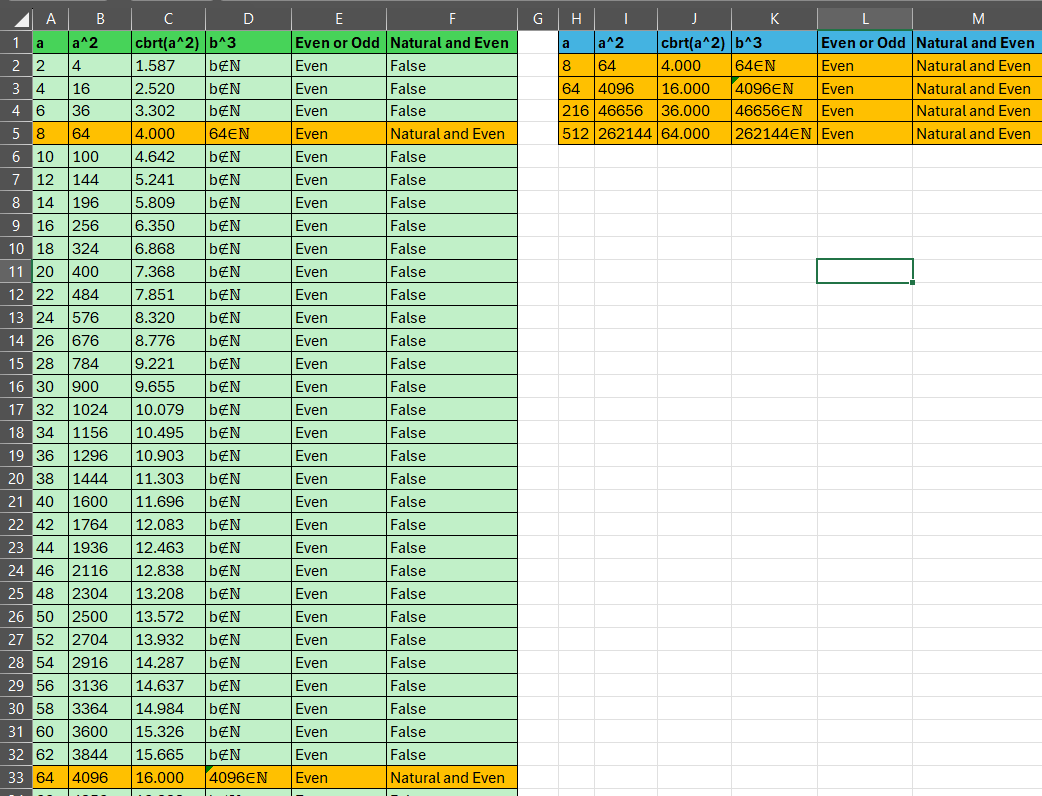
\includegraphics[width=\textwidth]{s.png}

\end{center}

\newpage

\subsection{Know-Show Table (\( a^2 = b^3 \) and \( a \) even \( \implies 4 \mid a \))}

\begin{center}
    \begin{tabular}{|p{.1\textwidth}|p{.6\textwidth}|p{.2\textwidth}|}
    \hline
    \textbf{Step} & \textbf{Know} & \textbf{Reason} \\
    \hline
        P1 & \( a^2 = b^3 \) & Hypothesis \\
    \hline
        P2 & \( a \) is even (\( a = 2k \)) & Hypothesis \\
    \hline
        P3 & \( (2k)^2 = b^3 \) & Substitution \\
    \hline
        P4 & \( 4k^2 = b^3 \) & Algebra \\
    \hline
        P5 & \( b \) is even (\( b = 2m \)) & Cubes divisible by 4 imply base divisible by 2 \\
    \hline
        P6 & Substituting \( b = 2m \): \( 4k^2 = (2m)^3 \) & Substitution \\
    \hline
        P7 & \( 4k^2 = 8m^3 \) & Algebra \\
    \hline
        P8 & \( k^2 = 2m^3 \) & Divide by 4 \\
    \hline
        P9 & \( k \) is even (\( k = 2n \)) & Squares divisible by 2 imply base divisible by 2 \\
    \hline
        Q1 & \( a = 4n \) & Substituting \( k = 2n \) into \( a = 2k \) \\
    \hline
    \textbf{Step} & \textbf{Show} & \textbf{Reason} \\
    \hline
    \end{tabular}
\end{center}

\newpage

\subsection{First Draft of Proof}

\begin{proof}
    Assume \( a^2 = b^3 \), and \( a \) is even. Then there exists an integer \( k \) such that \( a = 2k \). Substituting into \( a^2 \), we get:
    \[
    a^2 = (2k)^2 = 4k^2
    \]
    By the hypothesis \( a^2 = b^3 \), we know \( b^3 = 4k^2 \). Since \( b^3 \) is divisible by 4, \( b \) must be even. Let \( b = 2m \) for some integer \( m \). Substituting into \( b^3 \), we get:
    \[
    b^3 = (2m)^3 = 8m^3
    \]
    Thus:
    \[
    4k^2 = 8m^3
    \]
    Dividing both sides by 4, we find:
    \[
    k^2 = 2m^3
    \]
    Since \( k^2 \) is even, \( k \) must also be even. Let \( k = 2n \) for some integer \( n \). Substituting into \( a = 2k \), we get:
    \[
    a = 2(2n) = 4n
    \]
    Therefore, \( a \) is divisible by 4.
\end{proof}

\newpage

\subsection{Second Draft of Proof}

We aim to prove the following proposition:

\textbf{Proposition:} Let \( a, b \in \mathbb{N} \). If \( a^2 = b^3 \) and \( a \) is even, then \( 4 \mid a \).

\begin{proof}
    Assume \( a^2 = b^3 \), and \( a \) is even. Since \( a \) is even, there exists an integer \( k \) such that \( a = 2k \). Substituting \( a = 2k \) into \( a^2 \), we get:
    \[
    a^2 = (2k)^2 = 4k^2.
    \]

    By the hypothesis \( a^2 = b^3 \), it follows that:
    \[
    b^3 = 4k^2.
    \]

    Since \( b^3 \) is divisible by \( 4 \), \( b \) must also be even. Let \( b = 2m \) for some integer \( m \). Substituting \( b = 2m \) into \( b^3 \), we have:
    \[
    b^3 = (2m)^3 = 8m^3.
    \]

    Thus, the equation becomes:
    \[
    4k^2 = 8m^3.
    \]

    Dividing both sides by \( 4 \), we find:
    \[
    k^2 = 2m^3.
    \]

    Since \( k^2 \) is even, \( k \) must also be even. Let \( k = 2n \) for some integer \( n \). Recalling that \( a = 2k \), we substitute \( k = 2n \) into the expression for \( a \), and we have:  
    \[
    a = 2(2n) = 4n.
    \]

    Hence, \( a \) is divisible by \( 4 \), which proves the proposition that if \( a^2 = b^3 \) and \( a \) is even, then \( a \) must be divisible by \( 4 \).
\end{proof}

\newpage

\subsection{Reflection}

\begin{itemize}
    \item Initially, the proof was correct, but certain steps were less explicit. For example, it needed clearer justification for why \( b^3 \) being divisible by 4 implies \( b \) is even.
    \item The second draft improved these explanations, making the reasoning more direct and ensuring each step was justified.
    \item The final draft streamlined the logic, referenced prior results explicitly, and presented a fully rigorous and clear argument that \( a \) must be divisible by 4.
\end{itemize}


%------------Bibliography -------------

\begin{thebibliography}{9}
 \bibitem{Sund21} Sundstrom, T., \emph{Mathematical Reasoning: Writing and Proof}, Version 3,  Creative Commons, 2020.
 \bibitem{Flower08} Image source: \url{https://zollicoff.net/digital-art/} (my personal website)
\end{thebibliography}
\addcontentsline{toc}{section}{References}

\end{document}
